\chapter{Introdução} \label{ch:introduction}
Tendo em vista a necessidade de aspiração em piscinas e a crescente onda de automação residencial, observou-se a oportunidade de produzir um equipamento para realizar tal tarefa automática de piscinas \cite{kanno2014}.

Considerando o alto custo de aquisição de equipamentos modernos, internacionais e a grande demanda por serviços de higienização de piscinas, e o fato de que no Brasil não há empresas que desenvolvam este produto (há apenas revendedoras), o desenvolvimento do Clean Pool Robot permitirá a aplicação do conceito de automação a ambientes residenciais e a redução dos gastos com a contratação de um serviço terceirizado. As principais vantagens na utilização do Clean Pool Robot são:

\begin{itemize}
\item Retirar detritos do fundo da piscina que não foram alcançados por outros meios;
\item Mover a água ao passo que limpa as superfícies, melhorando a sua circulação;
\item Produzir um produto nacional que possui valor de mercado mais acessível.
\end{itemize}

Em uma pesquisa realizada pela equipe, verificou-se que a massa dos robôs que limpam piscinas variam de 8 Kg até 25 Kg e custam entre R\$ 2.000,00 e R\$ 16.000,00. O \cpr tem massa de aproximadamente 10kg e custará em torno de R\$ 7.000,00, preço mediano entre os concorrentes. Para a escolha de um limpador de piscinas automático, pequenas diferenças de especificação devem ser consideradas no momento da aquisição do aparelho, como por exemplo, ciclo de limpeza e taxa de filtragem. O ciclo de limpeza determina o intervalo de tempo em que o robô trabalha antes de se desligar automaticamente e a taxa de filtragem é determinada pela quantidade de água filtrada em uma hora, que é expressa em litros por hora (LPH). No caso do \cpr tem um ciclo de limpeza de 5h, tempo necessário para limpar uma piscina curta (semiolímpica).

O \cpr estará lidando basicamente com um corpo imerso em um líquido. Deste modo, o corpo estará essencialmente sob ação de duas forças: empuxo e peso.  Empuxo ocorre quando um corpo imerso na água parece ter se tornado mais leve devido a uma força, exercida pelo líquido sobre o corpo, vertical e para cima, que alivia o peso do corpo. Já o peso é devido à interação com o campo gravitacional da Terra.

Quando um corpo está totalmente imerso em um líquido, podemos ter as seguintes situações:

\begin{itemize}
\item Se ele permanecer parado no ponto onde foi colocado, a intensidade da força de empuxo é igual à intensidade da força peso;
\item Se ele afundar, a intensidade da força de empuxo é menor do que a intensidade da força peso;
\item Se ele for levado para a superfície, à intensidade da força de empuxo é maior do que a intensidade da força peso.
\end{itemize}

Como o robô realiza a limpeza do fundo da piscina, este deve estar afundado, ou seja, a intensidade da força de empuxo deverá ser menor do que a intensidade da força peso.

\section{Objetivos do Projeto}
Construir um robô capaz de realizar a remoção de sujeiras depositadas no fundo de piscinas por meio da aspiração e filtragem das impurezas. Os objetivos específicos são:

\begin{itemize}
\item Realizar aspiração automática dos resíduos decantados por meio da sucção e filtragem;
\item Submergir de forma independente;
\item Movimentar-se ao longo do fundo da piscina.
\end{itemize}

\section{Estrutura do Relatório}
A organização do projeto foi dividido em dois grupos: o grupo de estrutura e o grupo de lógica. Ambos os grupos se relacionam e tem trabalhado em conjunto. O diagrama abaixo apresenta a interação entre os grupos e as diversas engenharias que os compõem.
\par
  \begin{figure}[h]
    \centering
    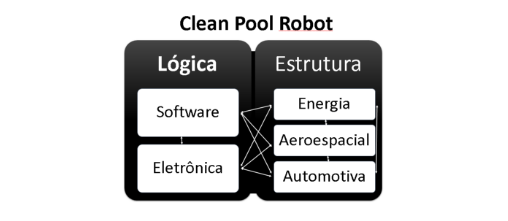
\includegraphics[width=0.8\textwidth]{figures/technical-div-project.png}
    \caption{Divisão técnica do projeto em dois segmentos.}
    \label{fig:technical-div-project}
  \end{figure}
  \FloatBarrier
\par
Apesar da divisão em duas grandes equipes, os membros interagiram de forma a preencher os requisitos e parâmetros solicitados por meio de documentos compartilhados via Google drive, ou por mensagens em grupos de conversa privados, utilizando-se do \textsf{WhatsApp}.

Nos próximos itens do relatório estão a visão geral no nosso produto, onde apresenta-se o \textit{design}, os sistemas que o compõem, os indicadores e a estimativa de custo. Em seguida tem-se o dimensionamento de cada componente. Por fim, a montagem do protótipo e os testes realizados.
